\documentclass[dvipsnames,svgnames,beamer]{beamer}

\usetheme{Boadilla}
%\usecolortheme{seahorse}

\usepackage[utf8]{inputenc}

\usepackage{cancel}

\usepackage{lib}

\setbeamercovered{invisible}

\setbeamertemplate{navigation symbols}{}

\setbeamertemplate{footline}{\hfill\insertframenumber\hfill\vspace{3mm}}

\title{Expanding the herd Memory model checker}

\author{Simon Colin}

\date{\today}

\begin{document}

\begin{frame}
	\titlepage
\end{frame}

\begin{frame}{Weak memory models}

	IBM Power and ARM mutliprocessors have highly relaxed memory models
	\vfill
	Relaxed memory models mean unexpected behaviors appear on concurrent programs	
	\vfill
	Interested in what behaviors are allowed
	
\end{frame}

\begin{frame}{Memory events}

	Programs are made of instructions
	\vfill
	Instructions involve memory events : reads from and writes to the shared memory
	\vfill
	We study these memory events

\end{frame}

\begin{frame}{weak memory models}

	\vfill
	\vfill
	Weak memory models allow a number of behaviors\begin{itemize}
	\item out of order execution
	\item speculative execution
	\item writes don't become visible to every thread at the same time
	\end{itemize}
	\vfill
	Fortunately, there are means to restore ordering
	\vfill

\end{frame}

\begin{frame}[fragile]{litmus tests}

	A litmus test is a short parallel program and an assertion about the result
	\begin{tabular}{p{4cm} p{4cm}}
	\begin{verbatim}
	Thread 0
	x = 1;
	y = 1;
	\end{verbatim} &
	\begin{verbatim}
	Thread 1
	while(y = 0) {}
	r1 = x;
	\end{verbatim}
	\end{tabular}
	\vfill
	We use them to find out about the possible behaviours of machines

\end{frame}

\begin{frame}

	Executions are a set of events and relations
	\begin{figure}[b]
	\centering
	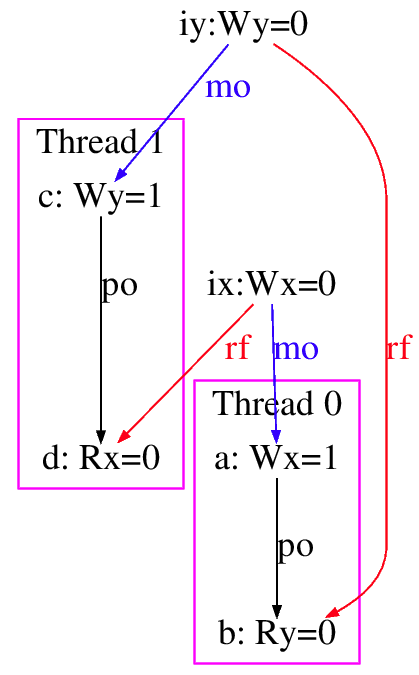
\includegraphics[width=4.5cm]{exec}
	\end{figure}

\end{frame}

\begin{frame}{RC11}

	\vfill
	\begin{itemize}
	\item $\hb ; \eco ^?$ is irreflexive. \hfill (coherence)
	\item $\rmw \cap (\rb ; \mo) = \emptyset$. \hfill (atomicity)
	\item $\psc$ is acyclic. \hfill (sequential-consistency)
	\item $\po \cup \rf$ is acyclic. \hfill (no-thin-air)
	\end{itemize}
	\vfill

\end{frame}

\begin{frame}{Herd}

	
	\begin{itemize}
	
	\item .cat file into a check
	\item litmus test into executions + constraints
	\item compute every combination of $\rf$ and $\po$ for each execution
	\item keep only the ones consistent with the model
	\item print the results to the user
	
	\end{itemize}

\end{frame}

\end{document}